\documentclass[11pt, a4paper]{article}

%\usepackage[T1]{fontenc}
%\usepackage{fullpage}

\usepackage[utf8]{inputenc} % comment when using lualatex
\usepackage[italian]{babel} % lingua e a-capo-sillabato
\usepackage{graphicx}
\usepackage[hidelinks]{hyperref,xcolor} % link di pagina
\usepackage[bottom]{footmisc} % note appiccicate al fondo della pagina
\usepackage{float} % per posizionamento immagini
\usepackage{amsthm}
\usepackage{fancyhdr}
\usepackage[font=small,labelfont=bf]{caption} % small font for caption (and bold Figure word)

\pagestyle{fancy}
\fancyhf{}% Clear header/footer
\fancyhead[C]{\footnotesize\textit{Documento:} D1 \hfill SleepCode \hfill \textit{Versione:} 2.3}
\renewcommand{\headrule}{{\color{red!70}\rule{\textwidth}{2pt}}}
\setlength{\headheight}{22pt}

%\pagestyle{myheadings}
%\markright{John Smith\hfill On page styles\hfill}

\renewcommand\UrlFont{\color{blue}\rmfamily}

\theoremstyle{definition}

\newtheorem{funcreq}{RF} %% numerazione dei requisiti funzionali
\newtheorem{nonfuncreq}{RNF} %% requisiti non funzionali
\newtheorem{backend}{BE}
\newtheorem{frontend}{FE}

\title{Analisi dei Requisiti}

\author{Raffaele \textsc{Castagna}\\
Alberto \textsc{Rovesti}\\
Zeno \textsc{Saletti}}

\newcommand{\groupNumber}{G17}


% —

% Web address for the project (if any)
% \newcommand{\homepage}{\url{https://www.}}

% data
\date{\today}

\makeatletter{}

% IL PREAMBOLO FINISCE QUI %%%%%%%%%%%%%%%%%%%%%%%%%%%%%%%%%%%%%%%%%%%%%%%%%%%%






\begin{document}

% La pagina di copertina si trova in un file .tex a parte
% NON MODIFICARE QUESTO COMANDO!!!
\begin{titlepage}
\newcommand{\HRule}{\rule{\linewidth}{0.3mm}} % Defines a new command for horizontal lines, change thickness here
\center % Centre everything on the page

%------------------------------------------------
%	Logo
%------------------------------------------------

\includegraphics[width=0.3\textwidth]{materiale/UniTrento_logo_ITA_colore.png}\\[0.5cm]
%------------------------------------------------
%	Headings
%------------------------------------------------
\textsc{\Large Dipartimento di Ingegneria\\e Scienza dell'Informazione}\\[1.5cm]

{\Huge\textbf{Sleep Code}}\\[0.5cm]
\textsc{\large Progetto per il Corso di Ingegneria del Software}\\
\textsc{\large Anno Accademico 2023-2024}\\[0.5cm]

%------------------------------------------------
%	Title
%------------------------------------------------

\HRule\\[0.4cm]
{\huge\bfseries \@title}\\[0.1cm]
\HRule\\[1cm]

\begin{minipage}{\textwidth}
\begin{flushleft}
\textit{Descrizione:} documento di analisi dei requisiti funzionali, non funzionali, front-end e back-end.
\end{flushleft}
\end{minipage}\\[1.5cm]


\begin{minipage}{0.4\textwidth}
\begin{flushleft}
\large
\textit{Numero documento:} D1
\end{flushleft}
\end{minipage}
\begin{minipage}{0.4\textwidth}
\begin{flushright}
\large
\textit{Versione documento:} 2.4
\end{flushright}
\end{minipage}\\[1.5cm]

%------------------------------------------------
%	Author(s)
%------------------------------------------------
\begin{minipage}{0.4\textwidth}
\begin{flushleft}
\large
\textit{Membri del gruppo:}\\
\@author % Your name
\end{flushleft}
\end{minipage}
~
\begin{minipage}{0.4\textwidth}
\begin{flushright}
\large
\textit{Numero gruppo: }
\groupNumber
\end{flushright}
\end{minipage}

% 	If you don't want a supervisor, uncomment the two lines below and comment the code above
% 	{\large\textit{Author(s)}}\\
% 	\@author % Your name

%------------------------------------------------
%	Date
%------------------------------------------------

\vfill\vfill
\textit{Ultima revisione:}
{\@date}

\end{titlepage}

\tableofcontents


\newpage
\section{Introduzione}
\subsection{Scopo del documento}
Le informazioni contenute in questo documento concorrono ad esporre l'analisi
dei requisiti relativa al progetto \textit{SleepCode}. In particolare, dopo
aver specificato gli obiettivi e il pubblico di riferimento, verranno definiti i requisiti
funzionali e non funzionali; verrà presentata una proposta di design di
front-end; infine saranno riportati i servizi esterni di back-end coi quali il
sistema dovrà interagire.


\subsection{Obiettivo del progetto}
Il progetto proposto si prefigge, come scopo fondante, di fornire alla comunità
di giovani informatici un servizio online di:
\begin{itemize}
    \item \textit{esercitazione} mirata alla programmazione e alla progettazione
    di piccoli algoritmi risolutivi, mediante la scrittura di codice;
    \item \textit{raccolta} di problemi attinenti.
\end{itemize}

\subsection{Pubblico di riferimento ed esigenze}
Il servizio vuole rendersi utile soprattutto a coloro che sono coinvolti
in percorsi di studio attinenti all'ambito informatico, ma specialmente anche
a chiunque desideri cimentarsi nella risoluzione di piccoli problemi di
programmazione; pertanto ci si aspetta che chiunque desideri usufruire del
servizio possieda almeno le conoscenze basilari della programmazione. Esempi
di queste nozioni pregresse, che tuttavia non devono necessariamente essere ampie e approfondite per utilizzare il servizio\footnote{Gli utenti più esperti possono indubbiamente trarre vantaggio dal loro bagaglio culturale per
approcciarsi con maggior facilità al servizio.}, sono: cosa si intende per
algoritmo e linguaggio di programmazione, familiarità nell'uso di qualche
linguaggio di programmazione, tipi e strutture di dati più comuni.

Di fatto, il progetto che verrà sviluppato ha come scopo principale di
creare una piattaforma accessibile online a singoli utilizzatori che
desiderano esercitarsi, valutare e approfondire le personali
conoscenze e abilità di \textit{problem solving} legate alla programmazione,
insieme all'archiviazione di nuovi problemi da rendere disponibili a coloro
che intendono usufruire del servizio.
D'ora in avanti, in questo e nei successivi documenti, questo pubblico di
individui appena descritti verrà indicato con il termine \textit{utenti}.

\newpage
\section{Requisiti funzionali}
Vengono di seguito elencati i requisiti funzionali (RF)
del progetto. Ogni sottosezione di questa parte del documento
risponde a diversi scopi precedentemente accennati, suddividendo
eventuali macro-funzionalità in requisiti minori nel caso di obiettivi
di più ampia portata.
\\\\
\noindent Le funzionalità sono inoltre suddivise secondo alcuni livelli di accesso
degli utenti (di seguito in ordine "crescente"):
\begin{itemize}
    \item \textit{Utente anonimo} (Sezioni 2.1, 2.2, 2.3).
    \item \textit{Utente autenticato} (Sezione 2.4).
    \item \textit{Utente amministratore} (Sezione 2.5).
\end{itemize}
Si precisa che un utente presente ad un dato livello di accesso può usufurire
delle funzionalità disponibili a quel livello \textit{più} le funzionalità
presenti al livello inferiore. Non è invece possibile utilizzare le funzionalità
messe a disposizione a eventuali livelli superiori.

\begin{center}
\section*{Utente anonimo}    
\end{center}


\subsection{Accesso e autenticazione}


\begin{funcreq}
\label{signup}
\textbf{Registrazione\footnote{Si denoterà con l'aggettivo \textit{registrato} un qualsiasi
utente che abbia precedentemente effettuato la registrazione e pertanto dotato di un account.} }
I nuovi utenti devono poter registrarsi al servizio, ovvero creare un account che
richiede la compilazione dei seguenti campi:
\begin{itemize}
    \item Nome utente (\textit{username}).
    \item Indirizzo di posta elettronica (\textit{email}).
    \item Password: data la sensibilità di questo campo, è importante
    che siano rispettati i vincoli riportati in \textcolor{blue}{\underbar{\hyperref[legalpassword]{RNF \ref*{legalpassword}}}};
    inoltre, l'utente deve poter riscrivere la password per confermarla, in
    modo tale da rilevare eventuali errori di digitazione.
\end{itemize}
\end{funcreq}

\begin{funcreq}
\label{login}
\textbf{Login }
Il sistema deve permettere all'utente registrato di autenticarsi,
accedendo al proprio account, mediante l'inserimento dell'indirizzo
email e la password impostate in fase di registrazione. L'utente deve
essere notificato qualora non sia possibile concludere correttamente
l'operazione di login, quindi se l'email inserita non è associata ad alcun
account registrato in precedenza oppure se la password è errata;
è comunque possibile ritentare il login un numero illimitato di volte.
Effettuato il login, l'utente accede alle funzionalità del livello \textit{autenticato}.
\end{funcreq}

\begin{funcreq}
\label{google}
\textbf{Autenticazione Google }
L'utente deve poter registrarsi ed effettuare il login sulla piattaforma
utilizzando un account Google, qualora non intenda ricorrere al sistema di
autenticazione interno descritto precedentemente (\textcolor{blue}{\underbar{\hyperref[signup]{RF \ref*{signup}}}}, \textcolor{blue}{\underbar{\hyperref[login]{RF \ref*{login}}}}).
In caso di registrazione, oltre alle operazioni previste dal servizio Google
(come la scelta dell'indirizzo email), l'utente deve solo specificare un username.
\end{funcreq}

\begin{funcreq}
\label{savepassword}
\textbf{Recupero password }
L'utente registrato e anonimo deve poter recuperare la password del proprio
account qualora tale dato dovesse essere dimenticato in fase di login. La
procedura di recupero deve prevedere:
\begin{itemize}
    \item L'invio di un messaggio all'indirizzo email attualmente associato
    all'account dell'utente—l'email contiene un collegamento ipertestuale
    che reindirizza l'utente ad una pagina dedicata, sulla piattaforma, nella
    quale completare l'operazione di recupero.

    \item L'inserimento di una nuova password nella pagina dedicata. La password, come in fase di
    registrazione, deve essere confermata e conforme al \textcolor{blue}{\underbar{\hyperref[legalpassword]{RNF \ref*{legalpassword}}}}.
\end{itemize}
Il recupero deve essere accessibile a tutti gli utenti registrati mediante
sistema di credenziali interno (\textcolor{blue}{\underbar{\hyperref[signup]{RF \ref*{signup}}}}, \textcolor{blue}{\underbar{\hyperref[login]{RF \ref*{login}}}}),
e non riguarda gli utenti registratisi mediante autenticazione Google
(\textcolor{blue}{\underbar{\hyperref[google]{RF \ref*{google}}}}).
\end{funcreq}

\subsection{Consultazione dei problemi}

\begin{funcreq}
\label{probcatalogue}
\textbf{Consultazione del catalogo dei problemi }
Il servizio deve mettere a disposizione un insieme di problemi sui quali
l'utente possa esercitarsi. L'utente deve poter consultare un catalogo,
atto a raccogliere i quesiti, e navigare al suo interno. Deve quindi
essere possibile:
\begin{enumerate}
    \item Visualizzare tale catalogo, che mostra i campi \textit{descrittivi}
    di ogni problema elencato:
    \begin{itemize}
        \item \textit{Nome:} una parola chiave priva di spazi.
        
        \item \textit{Difficoltà:} i problemi sono categorizzati in base alla
        loro difficoltà. Vengono definiti tre livelli indicativi:
        bassa, intermedia, alta.
        
        \item \textit{Tags:} un insieme di parole chiave che individuano una
        o più aree di interesse affrontate nel problema (ad esempio ricerca,
        grafi, ordinamento, hashing, ecc.)

        \item \textit{Suggerimento:} viene messo a disposizione, per ogni
        problema nel catalogo, un video in cui vengono trattate nozioni che
        possono aiutare ad affrontare il problema, suggerendo quindi all'utente un
        possibile approccio all'elaborazione della soluzione specifica del
        problema.
    \end{itemize}
    
    \item Cercare uno o più problemi specifici mediante ricerca filtrata per campi.
    Ai fini della consultazione del catalogo, i filtri applicabili riguardano i
    campi \textit{nome, difficoltà, tags}.

    \item Selezionare dal catalogo un problema specifico, cosicché
    il contenuto dell'intero problema possa essere visionato per mezzo
    delle funzionalità di cui al \textcolor{blue}{\underbar{\hyperref[seeproblem]{RF \ref*{seeproblem}}}}.
\end{enumerate}
\end{funcreq}

\begin{funcreq}
\label{seeproblem}
\textbf{Consultazione di un problema }
Deve essere fornito un visualizzatore che mostra le informazioni del
problema precedentemente selezionato dal catalogo. La visualizzazione
deve rendere disponibile alla vista dell'utente i contenuti del
problema (\textit{dati strutturali}):
\begin{itemize}
    \item Un titolo.

    \item Un testo, scritto prevalentemente in linguaggio naturale,
    che descrive uno scenario che richiede di essere risolto per mezzo
    di un algoritmo. Eventuali immagini e proposizioni matematiche
    possono accompagnare i testi.

    \item Almeno due esempi di input insieme al relativo output corretto,
    che mostra il risultato atteso\footnote{Non si devono confondere questi \textit{esempi}
    con i \textit{test cases} (\textcolor{blue}{\underbar{\hyperref[test]{RF \ref*{test}.2}}})}.
\end{itemize}
Qualora l'utente desideri consultare il problema, vengono contemporaneamente
messe a dispoizione le funzionalità di cui al \textcolor{blue}{\underbar{\hyperref[exesession]{RF \ref*{exesession}}}}.
\end{funcreq}

\subsection{Esercitazione}
\begin{funcreq}
\label{exesession}
\textbf{Effettuare un'esercitazione }
L'utente deve poter scegliere dal catalogo il problema desiderato e cominciare
a risolverlo. L'esercitazione deve avvenire in una vista apposita, dove
l'utente deve poter disporre di tutti gli strumenti necessari alla risoluzione
del problema, accedendo alle seguenti funzionalità:
\begin{enumerate}
    \item Visualizzare il contenuto dell'esercizio (\textcolor{blue}{\underbar{\hyperref[seeproblem]{RF \ref*{seeproblem}}}}).
    
    \item Visualizzare i test cases (\textcolor{blue}{\underbar{\hyperref[test]{RF \ref*{test}.2}}}).

    \item Essere al corrente di quale linguaggio di programmazione sia
    attualmente attivo per la scrittura di codice. Deve altresì essere 
    possibile selezionare uno dei linguaggi messi a disposizione dalla
    piattaforma\footnote{Per approfondimenti sulla disponibilità dei
    linguaggi, si veda \textcolor{blue}{\underbar{\hyperref[scalabilita]{RNF \ref*{scalabilita}.2}}}.}.

    \item Scrivere, sotto forma di codice nel linguaggio di programmazione
    scelto, l'algoritmo risolutivo del problema selezionato.

    \item Visualizzare il suggerimento (\textcolor{blue}{\underbar{\hyperref[probcatalogue]{RF \ref*{probcatalogue}.1}}}).
\end{enumerate}
L'esercitazione non è da confondersi come "sessione" registrabile dalla
piattaforma. In altre parole, l'utente può accedere all'area di esercitazione
(selezionando un problema) e abbandonarla in qualsiasi momento, ma nessun
dato cronologico o di altra natura, riguardo a tali azioni, deve essere memorizzato,
nemmeno nel caso in cui l'utente in questione sia autenticato.
\end{funcreq}


%\begin{funcreq}
%\label{sintax}
%\textbf{Correttezza sintattica del codice }
%L'utente deve poter verificare che il codice scritto sia corretto e in grando di essere eseguito in maniera appropriata.
%Quindi devono essere messe a disposizione le seguenti funzionalità:
%\begin{enumerate}
%    \item Compilazione del codice.
%    \item Visualizzazione di avvisi relativi a eventuali errori di compilazione
%    \textit{oppure} di compilazione andata a buon fine. In caso di errori
%    di scrittura, l'utente deve poter correggere tali errori riscrivendo
%    nell'area destinata al codice.
%\end{enumerate}
%\end{funcreq}

\begin{funcreq}
\label{test}
\textbf{Verifica della correttezza dell'algoritmo }
L'utente deve poter verificare la correttezza del codice scritto eseguendolo
e testandolo:
\begin{enumerate}
    \item Il codice deve essere eseguito sottoponendolo ad un certo numero
    di test cases, cioè fornendo opportune istanze di input e controllando
    l'output restituito. Il numero minimo di test cases per ogni problema
    corrisponde a 3.

    \item L'utente deve poter conoscere l'esito dei test case—per ognuno
    di questi, l'input e l'output atteso sono visibili. Inoltre, l'utente
    deve poter riscrivere e perfezionare l'algoritmo e sottoporre ripetutamente
    il codice ai test cases.

    Nel caso in cui l'esito dei test cases dovesse risultare negativo, l'utente
    viene avvisato senza fare riferimento agli errori commessi, siano essi
    relativi alla correttezza sintattica del codice oppure riguardanti la
    correttezza risolutiva dell'algoritmo.
\end{enumerate}
\end{funcreq}

\begin{funcreq}
    \textbf{Cronometro: }
    L'utente deve poter tenere traccia del tempo trascorso sulla piattaforma,
    ad esempio per conoscere il tempo impiegato per risolvere un problema.
    Quindi, l'utente deve poter avviare, interrompere e reimpostare a 0 secondi un
    cronometro. Il cronometro è disponibile in qualsiasi momento, sia durante
    la navigazione nel catalogo che durante la consultazione del problema
    e l'esercitazione.
\end{funcreq}
% cosa succede al cronometro se faccio altre cose tipo logout login e così via?

\newpage
\begin{center}
    \section*{Utente autenticato}
\end{center}

Nei seguenti requisiti funzionali, si suppone che l'utente appartenga al livello
di accesso \textit{autenticato}, qualora tale informazione dovesse essere omessa.
Si sottolinea nuovamente che l'utente autenticato eredita le stesse funzionalità
accessibili all'utente anonimo e descritte precedentemente.
\\
\begin{funcreq}
    \textbf{Metadati aggiuntivi }
    Oltre ai campi descrittivi specificati nel \textcolor{blue}{\underbar{\hyperref[probcatalogue]{RF \ref*{probcatalogue}.1}}},
    l'utente autenticato deve poter visualizzare e influenzare i seguenti dati aggiuntivi in
    ogni problema:
    \begin{enumerate}
        \item \textit{Stato:} i problemi risolti dall'utente devono essere contrassegnati,
        grazie alla disponibilità di questo ulteriore campo.
    
        \item \textit{Preferito:} l'utente che desidera tener traccia dei problemi
        per lui rilevanti deve poter contrassegnare tali problemi come \textit{preferiti}.
    \end{enumerate}
    Le informazioni riguardanti questi campi sono visibili all'utente autenticato,
    sia durante la consultazione del catalogo che del singolo problema. Si sottolinea
    che \textit{stato} e \textit{preferito} non sono attributi del problema in sé,
    bensì essi caratterizzazno la relazione tra un particolare utente autenticato e i
    problemi: ogni utente ha un proprio insieme di problemi preferiti e risolti,
    potenzialmente diverso da quelli di altri utenti registrati.
\end{funcreq}

\subsection{Gestione del profilo}
Indichiamo con il termine \textit{profilo} tutti i dati relativi all'attività
di un utente registrato e/o autenticato sulla piattaforma. Sono dunque inclusi
l'\textit{account} e i \textit{progressi} (\textcolor{blue}{\underbar{\hyperref[stats]{RF \ref*{stats}}}}).

\begin{funcreq}
\label{stats}
\textbf{Progressi } risolvendo i problemi, l'utente autenticato può migliorare
i propri \textit{progressi}.
\begin{enumerate}
    \item Il servizio deve prevedere il tracciamento dei progressi di ogni
    utente autenticato, incrementando il numero di problemi risolti ad ogni
    sessione di esercitazione andata a buon fine: con riferimento al
    \textcolor{blue}{\underbar{\hyperref[test]{RF \ref*{test}}}},
    dopo la risoluzione, il problema deve essere contrassegnato come
    \textit{risolto} (ciò modifica il campo \textit{stato} visibile nel catalogo
    e nell'area di consultazione ed esercitazione di quel problema).

    \item L'utente deve poter monitorare i propri progressi, accedendo ai dati
    seguenti:
    \begin{itemize}
        \item Il numero totale di problemi risolti.
        \item Il numero di problemi risolti suddivisi per difficoltà.
    \end{itemize}
\end{enumerate}
\end{funcreq}


\begin{funcreq}
\label{updateaccount}
\textbf{Aggiornamento account }
L'utente registrato e autenticato mediante il sistema di credenziali interno
deve poter modificare i dati identificativi del proprio account, ovvero indirizzo
email e password:
\begin{enumerate}
\item L'utente deve poter migrare ad un indirizzo email differente. La modifica
deve avvenire previo inserimento della password attualmente in uso.

\item L'utente deve poter modificare la password del proprio account.
La password può essere cambiata previo inserimento di quella attualmente
associata all'account. La nuova password deve essere digitata due volte
per conferma e deve rispettare quanto specificato dal
\textcolor{blue}{\underbar{\hyperref[legalpassword]{RNF \ref*{legalpassword}}}}.
\end{enumerate}
\end{funcreq}
    
\begin{funcreq}
\label{logout}
\textbf{Logout }
L'utente autenticato deve poter interrompere la sessione di accesso
al servizio. Questa procedura di \textit{logout} realizza il passaggio dell'utente
dallo stato autenticato a quello anonimo.
\end{funcreq}

\begin{center}
    \section*{Utente amministratore}
\end{center}

%Le funzionalità elencate di seguito sono usufruibili esclusivamente dall'utente
%amministratore. Inoltre, l'utente amministratore non può accedere alle funzionalità
%precedentemente descritte, cioè quelle caratteristiche dei livelli anonimo e autenticato.
\subsection{Gestione del catalogo dei problemi}

\begin{funcreq}
\textbf{Aggiungere un problema }
L'utente amministratore deve poter aggiungere un nuovo problema al catalogo.
La struttura del problema deve essere conforme a quanto descritto nel
\textcolor{blue}{\underbar{\hyperref[seeproblem]{RF \ref*{seeproblem}}}}
e, all'atto dell'inserimento nel catalogo, devono essere specificati i campi
elencati nel \textcolor{blue}{\underbar{\hyperref[probcatalogue]{RF \ref*{probcatalogue}.1}}}.

Inoltre, devono essere forniti almeno 3 test cases (questi saranno impiegati
come descritto dal \textcolor{blue}{\underbar{\hyperref[test]{RF \ref*{test}.1}}});
ogni test case consiste in un dato in input e il rispettivo output corretto.
\end{funcreq}

\begin{funcreq}
\textbf{Modificare un problema }
L'utente amministratore deve poter modificare sia i campi descrittivi del
problema, sia i dati strutturali (il contenuto).
\end{funcreq}

\begin{funcreq}
\textbf{Eliminare un problema }
L'utente amministratore deve poter eliminare i problemi dal catalogo.
\end{funcreq}

\newpage
\section{Requisiti non funzionali}
Vengono ora elencati i requisiti non funzionali (RNF) del servizio.

\subsection{Caratteristiche di sistema}

\begin{nonfuncreq}
\label{scalabilita}
\textbf{Scalabilità }
L'infrastruttura del servizio deve essere scalabile e aperta alle esigenze
derivanti dall'aumento di nuovi utenti. Questo requisito è motivato dalla
disponibilità online del servizio che verrà sviluppato. In particolare:
\begin{enumerate}
    \item L'infrastruttura del servizio deve essere adattabile a eventuali
    crescite nel numero di utenti, in modo da prevenire possibili cali di
    prestazioni eccessivi.

    \item Data l'eterogeneità di linguaggi di programmazione esistenti
    al momento della stesura di questo documento, è importante che il
    servizio sia in grado di accogliere con l'avanzare del tempo codici
    scritti in linguaggi differenti.
\end{enumerate}
\end{nonfuncreq}

\begin{nonfuncreq}
\label{compatibility}
\textbf{Compatibilità }
La piattaforma del servizio deve essere accessibile mediante le versioni
più recenti dei principali browser attualmente disponibili in commercio:
\begin{itemize}
    \item Chrome: 117.0.5938.150
    \item Firefox: 118.0.1
    \item Edge: 117.0.2045.60
\end{itemize}
\end{nonfuncreq}


\begin{nonfuncreq}
\textbf{Usabilità }
La piattaforma del servizio deve permettere all'utente di sfruttare le
funzionalità disponibili al proprio livello di accesso senza l'ausilio di
istruzioni scritte e verbose. L'intuitività dell'interfaccia deve essere
sufficiente a guidare l'utente nella realizzazione dei suoi scopi,
permettendo di venire a conoscenza di almeno il 90\% delle funzionalità del
servizio in meno di 30 minuti. 
\end{nonfuncreq}

\begin{nonfuncreq}
\textbf{Aspetto }
L'interfaccia deve presentarsi gradevole alla vista dell'utente, preferendo
gradazioni cromatiche scure e un contrasto sufficientemente equilibrato,
al fine di garantire la leggibilità e contribuire alla riduzione
dell'affaticamento della vista. Una motivazione a supporto di questo requisito
è il potenziale rischio di sessioni di navigazione eccessivamente prolungate sulla piattaforma.
\end{nonfuncreq}

%QUESTIONE LINGUA: dato che gli amministratori possono essere persone qualunque, chi garantisce che scriveranno testi e useranno video-suggerimento in ita/eng? specifichiamo una policy?
\begin{nonfuncreq}
\textbf{Lingua di sistema }
Il servizio viene erogato in lingua italiana.

%Altrettanto viene fatto per i
%testi dei problemi. I video relativi alla soluzione dei problemi possono
%essere in italiano oppure in inglese.
\end{nonfuncreq}

\begin{nonfuncreq}
\textbf{Prestazioni }
L'esperienza di utilizzo deve poter essere soddisfacente in relazione
ai livelli di prestazioni dei moderni siti web, purché l'utente utilizzi
il servizio in condizioni di connettività sufficienti. In particolare,
i tempi di reazione relativi a caricamenti e transizioni tra pagine non
deve eccedere, indicativamente, i 2 secondi.
\end{nonfuncreq}

\subsection{Affidabilità}

\begin{nonfuncreq}
\label{downtime}
\textbf{Downtime }
Il downtime annuo della piattaforma non deve eccedere gli intervalli di
tempo indispensabili a eventuali opere di manutenzione e aggiornamento
\textit{sui componenti interni al servizio}, evitando ove possibile
interruzioni di servizio inutilmente prolungate. Si prevede di non superare
un downtime del 2,7\% nel primo anno (10 giorni su 365, per un totale di 240
ore) dopo il lancio della piattaforma, per poi mantenere il rapporto al di
sotto del 0,85\% (circa 72 ore).
\end{nonfuncreq}

\begin{nonfuncreq}
\textbf{Disponibilità }
\label{disponibilita}
Il progetto sviluppato ha il 98\% di probabilità di non guastarsi entro le
prime 8.000 ore di funzionamento. La disponibilità dei servizi terzi, sui
quali il progetto si affida (database, contenuti multimediali), permette di
trascurare eventuali variazioni di tempo aggiuntive riguardanti le
interruzioni di servizio inattese.
\end{nonfuncreq}

\subsection{Privacy e sicurezza}

\begin{nonfuncreq}
\textbf{Privacy e trattamento dei dati }
Il servizio deve essere progettato e realizzato in ottemperanza delle
vigenti disposizioni di legge in materia di tutela della privacy e
trattamento dei dati:
\begin{enumerate}
    \item L'applicazione fornita dal servizio deve essere conforme
    al regolamento \href{https://www.garanteprivacy.it/documents/10160/0/Regolamento+UE+2016+679.+Arricchito+con+riferimenti+ai+Considerando+Aggiornato+alle+rettifiche+pubblicate+sulla+Gazzetta+Ufficiale++dell%27Unione+europea+127+del+23+maggio+2018}{\textcolor{blue}{\underbar{UE n.2016/679}}} (GDPR) per la protezione dei dati.
\end{enumerate}
\end{nonfuncreq}

\begin{nonfuncreq}
\textbf{Connessione sicura }
La comunicazione con il client deve essere protetta da protocolli
di sicurezza, come \texttt{https}, che consentano di preservare la
riservatezza dei dati scambiati tra piattaforma e client utente.
\end{nonfuncreq}

\begin{nonfuncreq}
\label{legalpassword}
\textbf{Password strength }
In tutti gli scenari nei quali è richiesta la creazione di una password,
la stringa inserita deve rispettare le seguenti caratteristiche:
\begin{itemize}
    \item Lunghezza compresa tra 8 e 64 caratteri.
    \item Contenere almeno una lettera maiuscola.
    \item Contenere almeno una lettera minuscola.
    \item Contenere almeno un numero.
    \item Contenere almeno un carattere speciale scelto tra i
    seguenti:
    \begin{center}
        \verb|! ? # $ % & @ * + . , ; : / - = _ \ ( ) [ ] { }|
    \end{center}
\end{itemize}
\end{nonfuncreq}

%\begin{nonfuncreq}
%\textbf{Integrità e operazioni su dati sensibili }
%L'integrità di dati sensibili dell'account, quali email ma soprattutto password,
%è garantita da opportune procedure di conferma e notifica all'utente.
%Data la natura di queste operazioni di sicurezza, i requisiti funzionali
%relativi alla gestione dei dati sensibili (RF \ref{signup}, RF \ref{savepassword},
%RF \ref{updateaccount}) provvedono a descrivere il comportamento del
%servizio nel caso di errori e incongruenze.
%\end{nonfuncreq}



\newpage
\section{Design front-end}
In questa sezione vengono presentati alcuni mock-up dell'interfaccia che
la piattaforma online espone all'utente.

\begin{frontend}
\textbf{Pagina di login }
\end{frontend}
\begin{figure}[H]
\centering
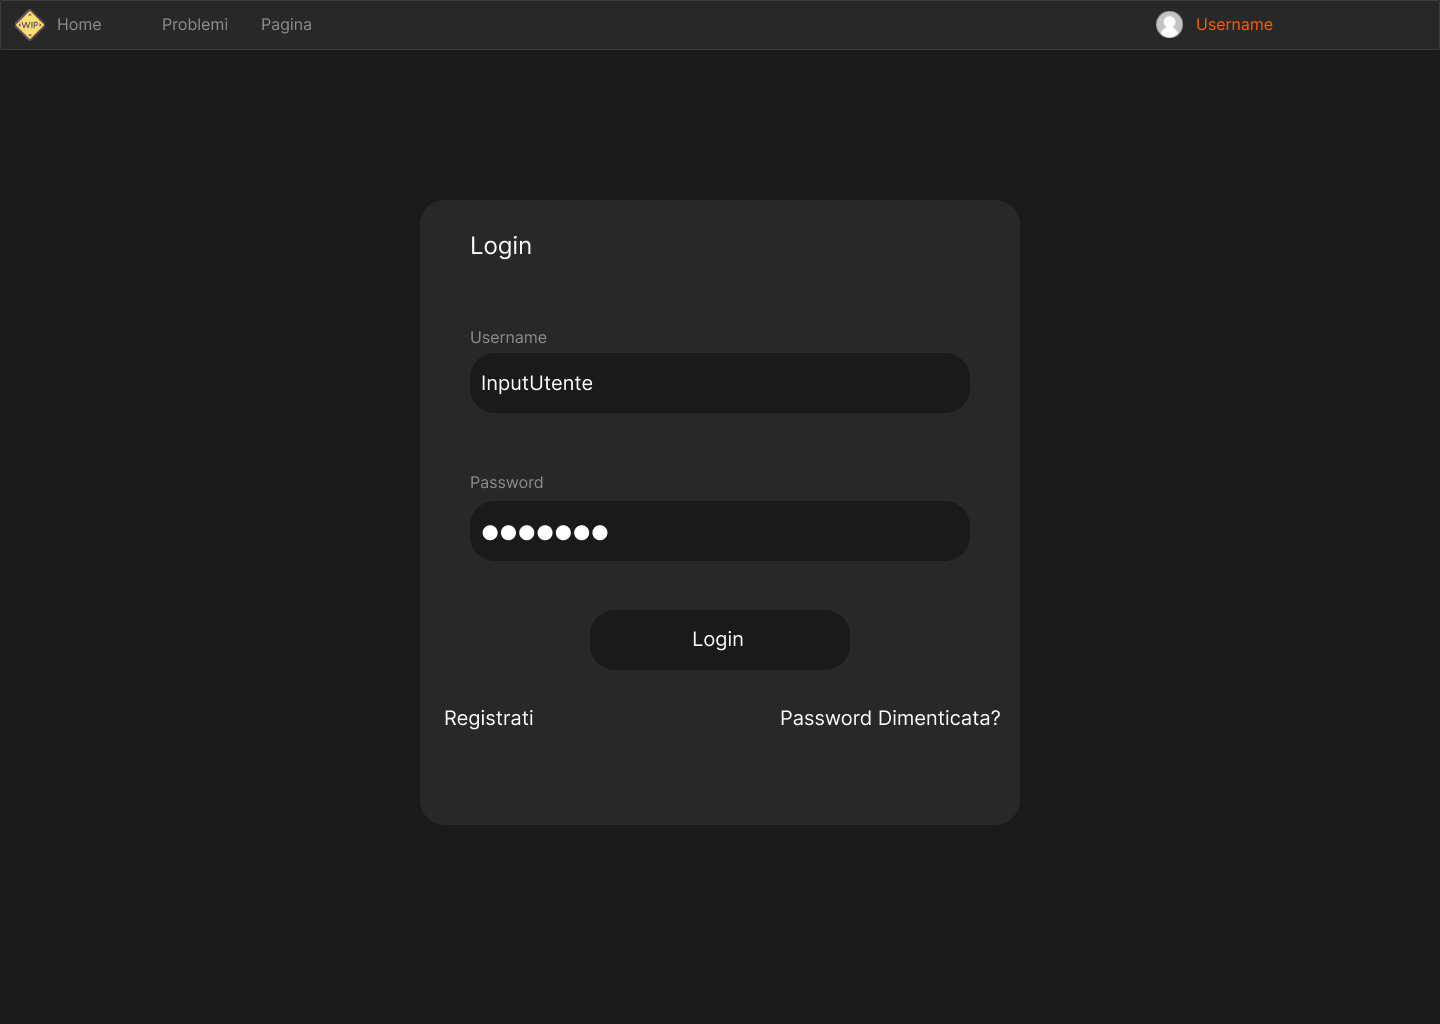
\includegraphics[scale=0.22]{materiale/immaginife/login.jpeg}
\end{figure}

\begin{frontend}
\textbf{Pagina di registrazione }
\end{frontend}
\begin{figure}[H]
\centering
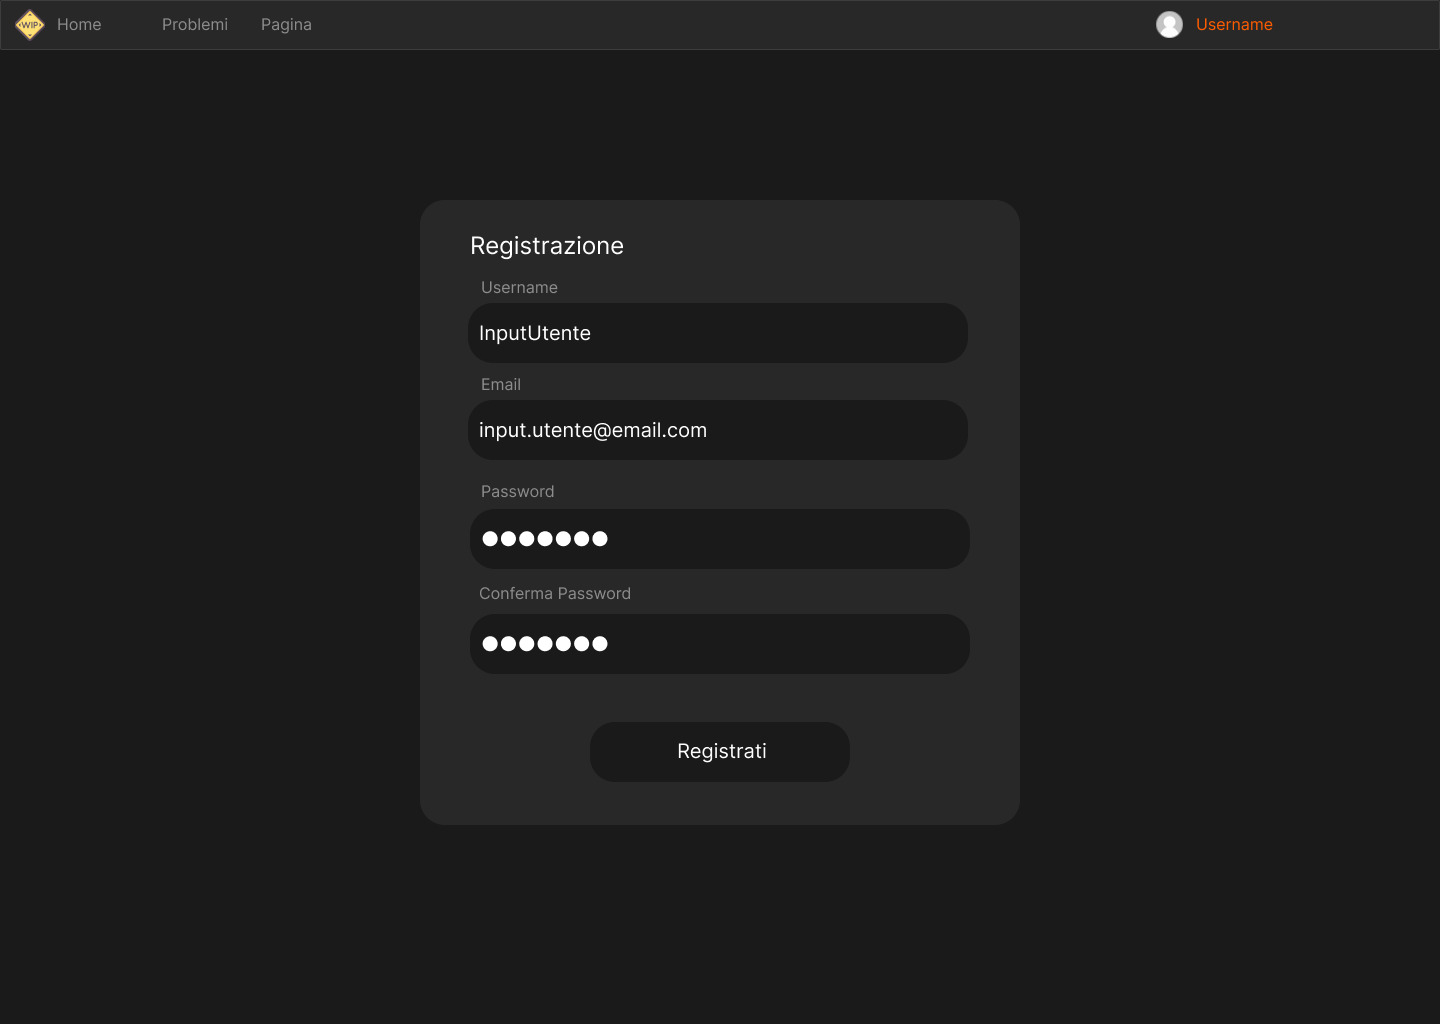
\includegraphics[scale=0.22]{materiale/immaginife/registrazione.jpeg}
\end{figure}

\newpage
\begin{frontend}
\textbf{Home page }
Il catalogo e il profilo utente, insieme a tutti i collegamenti che consentono
di usufruire della maggior parte delle funzionalità del servizio, sono
contenute in una pagina principale. Il seguente mock-up mostra la vista che si
presenta ad un utente autenticato (è presente il campo \textit{stato}, oltre all'icona
per contrassegnare i \textit{preferiti}).
\end{frontend}
\begin{figure}[H]
\centering
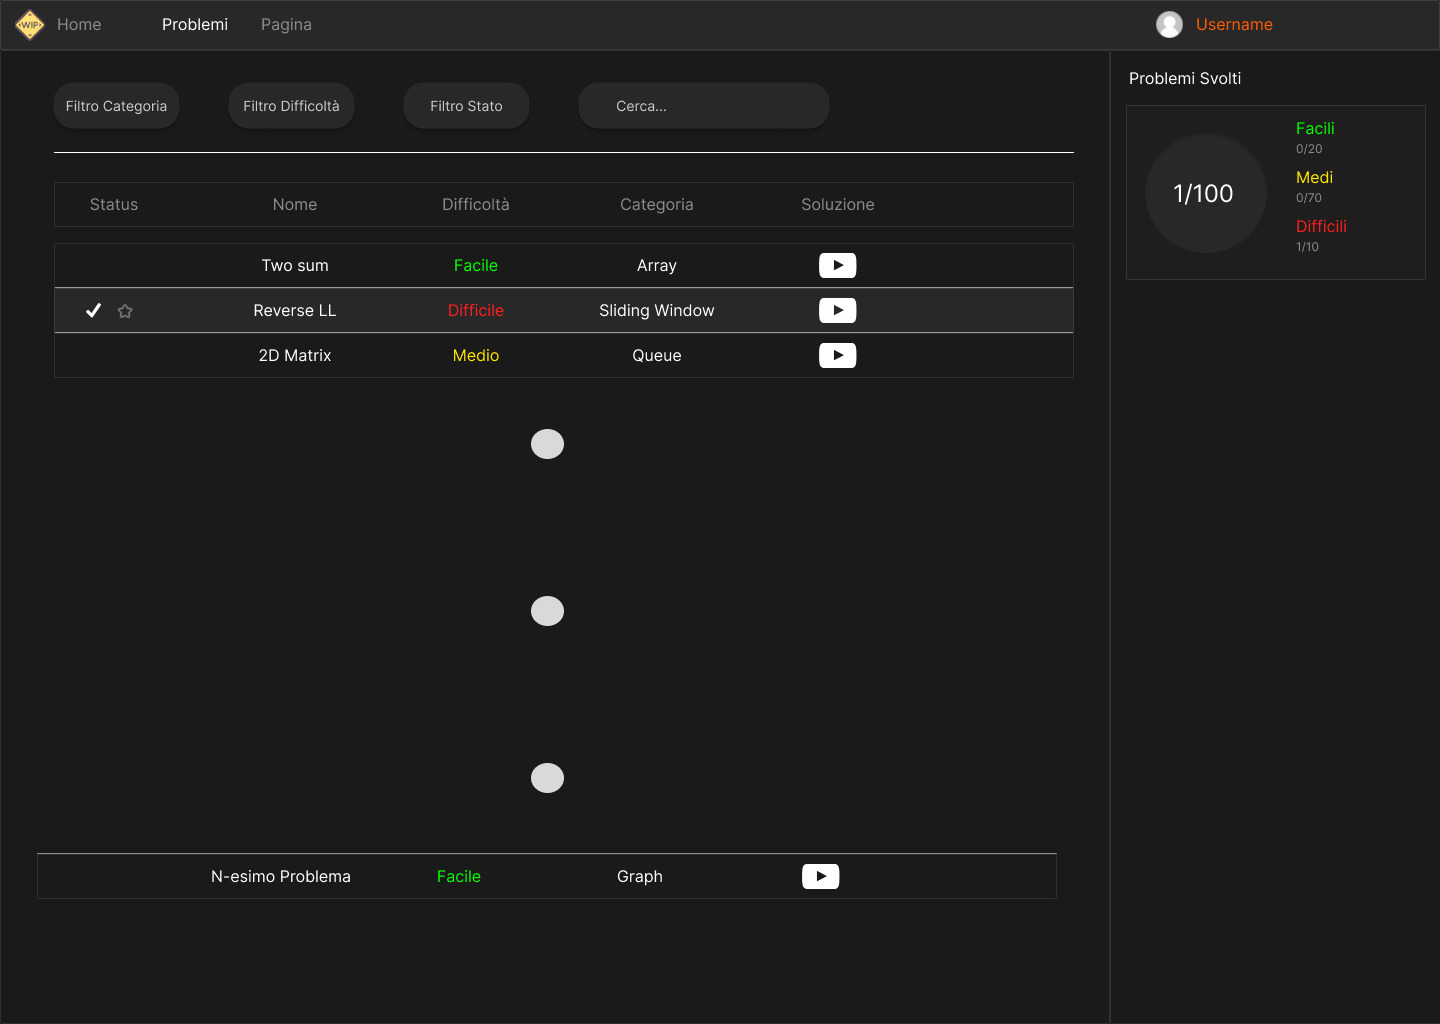
\includegraphics[scale=0.195]{materiale/immaginife/homecatalogo.jpeg}
\end{figure}

\begin{frontend}
\textbf{Pagina di esercitazione }
Una pagina dedicata raccoglie le funzionalità di consultazione dettagliata
del problema e risoluzione di quest'ultimo.
\end{frontend}
\begin{figure}[H]
\centering
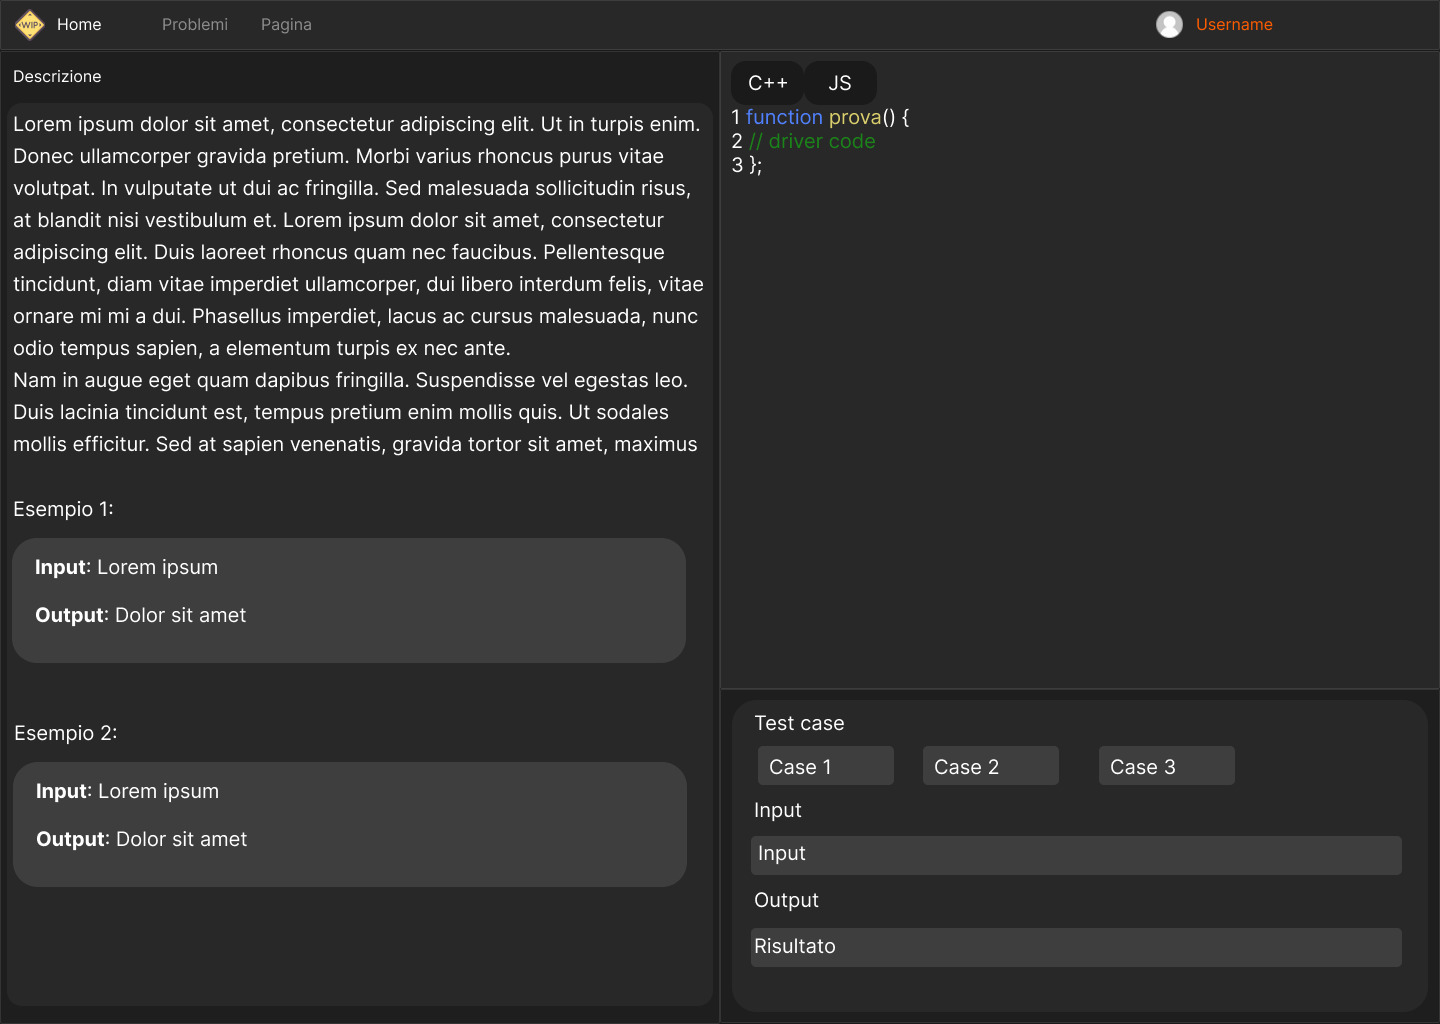
\includegraphics[scale=0.195]{materiale/immaginife/esercitazione.jpeg}
\end{figure}

\newpage

\begin{frontend}
\textbf{Editor del catalogo }
La seguente figura mostra l'interfaccia che si presenta ad un utente
amministratore nel momento in cui desidera modificare il catalogo dei
problemi.
\end{frontend}
\begin{figure}[H]
\centering
%\includegraphics[scale=0.5]{materiale/immaginife/boh.jpeg}
\end{figure}

\begin{frontend}
\textbf{Logout }
Un pulsante di logout è raggiungibile in ogni momento da parte dell'utente
autenticato.
\end{frontend}
\begin{figure}[H]
\centering
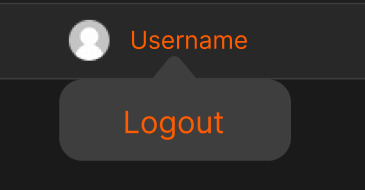
\includegraphics[scale=0.2]{materiale/immaginife/logout.jpeg}
\end{figure}

\newpage
\section{Design back-end}
Nella sezione seguente vengono elencati i servizi esterni con i quali
la piattaforma \textit{SleepCode} interagisce per funzionare
correttamente, o per ricevere supporto mirato a soddisfare i propri requisiti.
In Figura \ref{backend} viene riassunto l'insieme di questi servizi esterni
e il ruolo che essi svolgono nell'interazione, in ambito back-end (BE),
con il progetto da realizzare.

\begin{backend}
\textbf{Servizio di autenticazione alternativo }
L'utente può scegliere di registrarsi e accedere all'account sulla piattaforma
mediante un account Google. Questo servizio offre all'utente un meccanismo di
autenticazione alternativo al sistema di credenziali interno, realizzando quando
descritto in \textcolor{blue}{\underbar{\hyperref[google]{RF \ref*{google}}}}.
\end{backend}

\begin{backend}
\textbf{Contenuti multimediali }
Per reperire e riprodurre i video contenenti i suggerimenti dei problemi (\textcolor{blue}{\underbar{\hyperref[probcatalogue]{RF \ref*{probcatalogue}.1}}}),
il servizio si ricorre alla piattaforma YouTube.
\end{backend}

\begin{backend}
\textbf{Database }
La memorizzazione degli account degli utenti, dei problemi disponibili
nel catalogo e dei dati annessi si affida al servizio di database offerto
da Firebase.
\end{backend}

\begin{backend}
\textbf{Notifica via posta elettronica }
L'invio dei messaggi email, ai fini del recupero dell'account (\textcolor{blue}{\underbar{\hyperref[savepassword]{RF \ref*{savepassword}}}}), viene gestito da servizi di posta elettronica di terze parti.
\end{backend}
% possibili candidati: gmail

\begin{figure}[H]
\centering
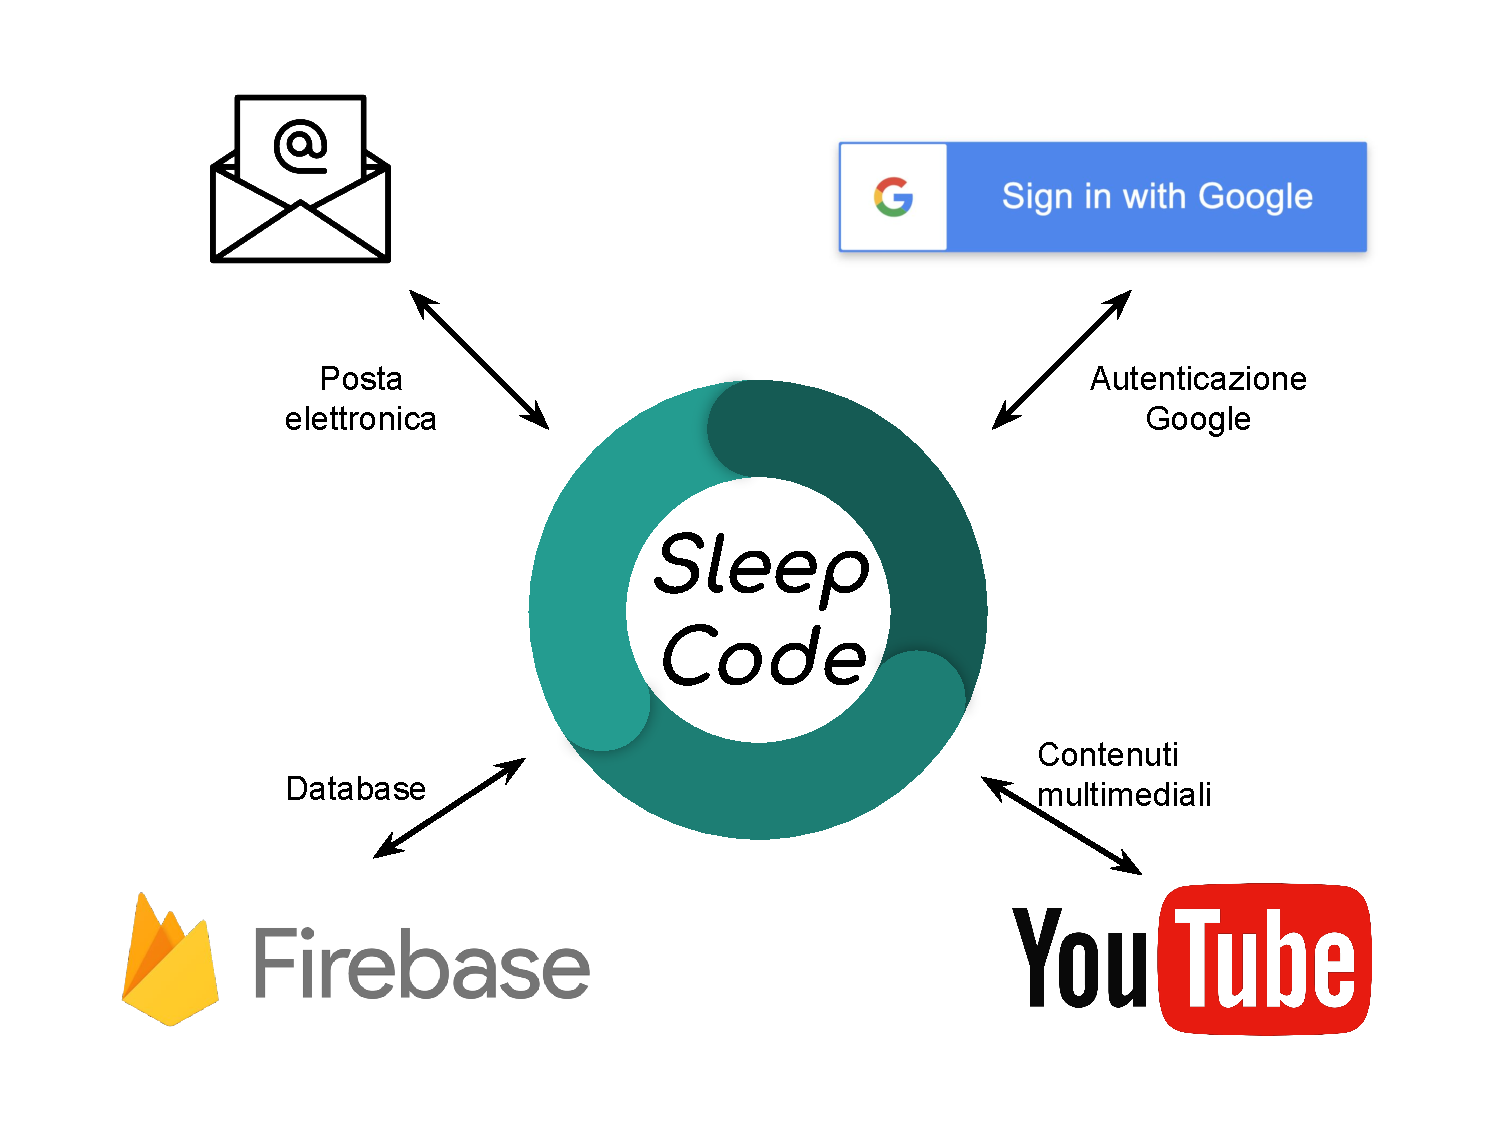
\includegraphics[scale=0.35]{materiale/immaginife/backend.pdf}
\caption{Diagramma di back-end con i servizi esterni su cui il progetto si appoggia}
\label{backend}
\end{figure}

%\newpage
%\section{Cronologia}
%Nella cronologia sono riportate le versioni del documento
%\begin{itemize}
%    \item \textit{Versione 1.0:} prima stesura definitiva.
%    \item \textit{Versione 2.0:} definizione dei livelli di accesso e conseguente estensione delle funzionalità.
%    \item \textit{Versione 2.1:} ridefinizione delle funzionalità del livello amministratore.
%    \item \textit{Versione 2.2:} eliminazione RF sulla correttezza sintattica del codice; aggiornato il ruolo amministratore.
%    \item \textit{Versione 2.3:} chiarificazioni sul ruolo e sulle funzionalità del cronometro.
%\end{itemize}

\end{document}